\documentclass{article}

\usepackage[utf8]{inputenc}
\usepackage[numbers]{natbib}
\usepackage{graphicx}
\usepackage{multirow}
\usepackage{enumitem}
\graphicspath{ {./images/} }

\title{SageSense : managing excessive smartphone use}
\author{Betrant Titus}
\date{March 2019}

\begin{document}
\maketitle


\begin{abstract}
    The smartphone is a wondrous device, and it's usage has been steadily on the rise since the turn of the last decade. These proclaimed benefits, such as the increase in productivity and the wide range of features that it offers are not without its caveats. Several studies have proven that the average increase in smartphone usage amongst users has been linked to deterioration of mental health\cite{bian2015linking,twenge2017have,ward2017brain}. Thus, it becomes very obvious that the pervasive adoption of these devices drags an increasing amount of people into mental health issues like depression and lethargy. The fact that such users aren't aware of such risks aggravates the problem. This paper attempts to tackle the aforementioned problem by proposing a solution, named SageSense, which aims to decrease excessive usage of smartphones. It is a smartphone application which connects to a wearable system that tracks the user's mental acuity and status, and helps the user limit smartphone use by suggesting a daily limit on the time he/she is able to use the device. SageSense proves to be more effective than its counterparts that utilize similar strategies to reduce smartphone usage, since it delivers dynamic and personalized usage limits based on the multiple inputs recorded by the wearable system that it connects to. It proves effective in curbing excessive and/or compulsive smartphone use, which resulted in a visible improvement in overall mental health amongst the users of the solution. This was confirmed with an analysis of brain wave activity of 420 users conducted before and after 60 days of continued usage of the application, out of which brain wave data of 381 (90.71\%) users indicated improvement in mental acuity, concentration, satisfaction and happiness, which in turn indicated positive trends in overall mental health.
    
    \textbf{KEYWORDS}: smartphone addiction, mental health, brain wave analytics, technostress
\end{abstract}


\newpage


\section{Introduction}

\paragraph{} Ever since its conception in the early 2000s, the smartphone has steadily grown to be a tool that its users have utilized to increase productivity. This was achieved by the plethora of features offered by these devices, rendering the users of such devices able to achieve a substantial increase in productivity. It's ability to provide content from the Internet has made it a device to easily consume media such as news, articles, videos, music and much, much more. All of these have fostered its adoption among humankind, as the number of smartphones in use amongst the total population of the world has always been on the increase since it was introduced into the world. Even if this seems something to be regarded positively when casting a cursory glance, a deeper foray into this subject shows that all is not well in this seemingly cheery world\cite{lee2014dark}. A substantial percentage of all the smartphone users are reported to be overdependent on their smartphones\cite{lopez2014prevalence, merlo2013measuring, lee2016dependency, davey2014assessment, eduardo2012mobile, koo2014risk}, and as the number of smartphone users increase, so do the number of such users. Such usage patterns lead to technostress\cite{brod1984technostress}, leading them on a declining slope of mental health and rendering these users prone to mental health issues such as mood swings, depression and lethargy.\cite{van2015modeling, lee2013relationship, choi2012influence, wang2014studentlife}

\paragraph{} This paper is an attempt to understand this problem further by building on past analyses and then trying to tackle the problem of excessive and/or compulsive usage of smartphones. We then proceed to introduce SageSense, our solution which consists of two subsystems:

\begin{itemize}
    \item an Android application that displays usage of the smartphone on a temporal basis (and additionally per-app usage) and provides lock-out timeframes based on automated analysis of the data collected from the second subsystem.
    \item an interlinked set of wearable devices which includhddband and a wristband, and the inbuilt sensors present in the smartphone (accelerometer, front-facing camera, touchscreen), which together collect data that includes brain wave activity, eye movements, and touchscreen interaction patterns.
\end{itemize}

\paragraph{} These subsystems work in tandem to record and analyze real-time data, based on which inferences can be made about the user's current state of mind and levels of mental acuity. This is then used to generate a dynamically generated lockout timeframe which the user is compelled to follow. The generation of the timeframe is adjusted according to the user's day-to-day usage patterns and mental health levels. This provides SageSense a clear advantage over the competition, giving it the ability to adapt to users by delivering lockout timeframes that provide the optimal improvement in the user's usage of his/her smartphone.

\paragraph{} Our solution, SageSense, provides an objectively better method by which a user can keep track of his/her smartphone usage patterns and decrease technostress by the method of adhering to the lockout timeframes regulated by the application. The effectiveness of the solution was analyzed with the help of a study of brain wave data collected from a fixed number of users (420 users) at two points in time:

\begin{itemize}
    \item before the user started using the application
    \item after the user completed 60 days of continued usage of the application
\end{itemize}

\paragraph{} This data was collected over a 24-hour period during the aforementioned points in time, which allowed us to analyze the difference in the user's mental health before using the application and after using the application. The analysis of this data ended with the conclusion that 90.71\% of users (381 users) showed noticeable improvement in overall mental health, which was indicated by increase in levels of mental acuity, concentration, satisfaction and happiness in general.

\paragraph{} We believe the following to be our contributions:

\begin{itemize}
    \item We conduct an analysis of brain-wave patterns on a multi-ethnic group of participants, and prove the hypothesis that excessive and/or compulsive smartphone usage has detrimental effects on mental health.
    \item We propose and implement a solution, SageSense, which provides an improvement over similar solutions, by providing the user with a dynamic and personalized timeframe in which the user is not allowed to use his/her smartphone.
    \item We confirm the effectiveness of the solution implemented by conducting an analysis on the brain wave activity of users before and after using the solution for a period of 60 days, and compare the changes in trends of brain-wave activity before using the application and after continued usage of the application for the specified time period.
\end{itemize}

\section{Related Work}

\paragraph{} Since the start of the current decade, researchers have been increasingly aware of the negative effects of the increase in smartphone usage\cite{perlow2012sleeping, twenge2018increases, international2011iarc}. However, there was no strong focus on any of the negative side effects of smartphone overuse. Studies that did explore the negative effects of smartphones stressed on topics such as physical health problems\cite{rebold2016impact, kim2015relationship, korpinen2013self, white2004risk, inal2015effects} or academic problems\cite{alfawareh2014smartphones, samaha2016relationships, kibona2015smartphones, kibona2015review, felisoni2018cell, hawi2016excel, choi2012influence}. Additionally, there was not enough scientific basis to claim that compulsive smartphone usage is a behavioral disorder relating to addiction. However, with the increasing reports of such overuse of these devices, addiction had to be redefined. Multiple studies\cite{grant2016expanding, young2004internet, sussman2011considering} attempted to redefine the same, and as a result, compulsive usage of smartphones became recognized as a behavioral addiction that does not require a consumable such as alcohol.

\paragraph{} There are multiple systems that provide solutions to the problem of smartphone overuse. Certain systems utilize manual intervention and/or third-party intervention to regulate smartphone usage\cite{ko2015nugu, ko2015familync, howells2016putting}. However, the pitfall of this design is that the control of the limiting factor is with user's loved ones, which can be overridden with necessary social engineering. To improve upon this method, certain systems transfer control to the user himself/herself. Such applications\cite{lee2016design, lochtefeld2013appdetox} are also fall short, since such applications are at the control of the user, whose choice of volunteering to follow the lockout may not be effective at all times. An alternative workaround to the problem is that an incentive could be offered for completion of certain tasks prescribed by the system\cite{runyan2013smartphone}. However, the problem is still not solved since the user can still choose to ignore the system altogether. Additionally, these applications deliver static usage/lockout timeframes, which may not be reflective of the gradual change that the user achieves in his/her smartphone usage patterns. Certain systems\cite{ko2016lock} also lockout the user in the presence of social gatherings, based on geolocation and event analysis, but this is a solution with an very specific trigger for lockout which is geared at increasing social interaction amongst smartphone users, which is not our focus, even if the system is a potent one.

\paragraph{} Thus, it is our objective to build a system which analyzes the state of the user to gauge the level of lockout that he/she requires, instead of depending on the user himself/herself or a third-party. Additionally, the system should be also reflective of the changes that happen to the user over time, such as the gradual improvement in the levels of smartphone usage. Thus, these timeframes that are devised in the system should change with respect to the such changes that occur i.e. these timeframes need to be dynamic.

\paragraph{} Additionally, our solution integrates brain-wave analysis and eye movement analysis to deliver personalized timeframes, which are not present in any application-based solutions present today. SageSense borrows from the concept of analysing the electrical signals transmitted in the brain i.e. brain-wave analysis\cite{da1991neural, buzsaki2006rhythms} using a wearable system which essentially tracks the brain-wave activity by delivering a real-time EEG (Electroencephalogram) which is analyzed\cite{sigl1994introduction}. We also utilize a standardized method of eye movement analysis\cite{ulmer1996process} to infer the levels of attentiveness and concentration of the user. This data is collectively used to understand the relative status of the user and deliver personalized and dynamic lockout timeframes.

\section{Experiments Conducted}

\paragraph{} We conduct two experiments; one in which we lay the groundwork for the problem and prove that excessive and/or compulsive use of smartphones has detrimental effect on mental health, and the next in which we test the effectiveness of SageSense and prove that this is indeed a viable, if not better solution to curbing excessive and/or compulsive smartphone usage.

\subsection{Experiment 1 : Validation of premise}

\paragraph{} We propose an experiment that utilizes a subset of features provided by SageSense (static lockout timeframes) to analyze and prove the hypothesis that excessive and/or compulsive use of smartphones serve as a catalyst in development of mental health disorders. The experiment, if successful, will display that users with no restriction in their smartphone usage will display sub-par mental health when compared to people who restrict their smartphone usage (voluntarily / non-voluntarily). To conduct this experiment, we run an analysis of brain-wave patterns on multi-ethnic subject groups, in which each group is subjected to a certain level of smartphone usage on a temporal basis. The required brain-wave data is collected from each participant daily for the total duration of the experiment (60 days), and a progressive comparison is made for each subject with data obtained thus on each day.

\subsubsection{Research Data}

\paragraph{} The experiment focuses on the variance in biological parameters pertaining to mental health, and as such is done with the help of data that is generated from continued usage of the smartphone application designed alongside the wearables that connect to it, which are discussed in detail later. The data collected include the following:

\begin{itemize}
    \item Brain waves, which include alpha, beta, gamma, delta and theta waves
    \item Eye movements
    \item Touchscreen interaction patterns and frequencies
\end{itemize}

\paragraph{} This data is collected from every participant on a daily basis for a period of 60 days, wherein the users are given lockout timeframes and are supposed to adhere to it, without any breaks in the timeframe provided. Such users are excluded from the study.

\paragraph{} We utilize \citeauthor{buzsaki2006rhythms}'s work\cite{buzsaki2006rhythms} on brain wave data to provide a set of guidelines that this experiment builds upon, which are as such:

\begin{itemize}
    \item Alpha waves correlate to the brain's state to learn and stay attentive.
    \item Alpha waves also correlate to tasks that require a high degree of coordination.
    \item Beta waves correlate to the brain's state of decision making.
	It also acts as another indicator of the focused state of mind.
    \item Gamma waves indicate the heightened state of mind i.e. a trance-like state or a mindful state of deep meditation.
    \item Delta waves indicate the state of 'drifting away' or 'dreaming' and also indicates the urge to sleep.
    \item Theta waves are indicators of multiple things; sleep, learning and heightened states can all be indicated with the same.
    \item The speed of eye movements provides a relative scale on the mental energy levels of the subject, which can be concurred with the levels of delta waves.
    \item The frequency of eye movements provides the relative scale of the attention span of the subject.
    \item Touchscreen interaction patterns are utilized to confirm the findings that are indicated with the given levels of brain waves at a certain instant of time.
\end{itemize}

\subsubsection{Experimental Setup}

\paragraph{} The framework for the experimental setup was provided by SageSense, whose feature of providing lockout timeframes (albeit utilized here on a fixed scale) allowed it to act as the central setup for data collection, with which the aforementioned data was recorded from the participants. The setup includes an Android application that runs on the participant's smartphone, and tracks the usage of the participant over time, and also maintains a history of the usage patterns for a defined number of days (which in this case was made to be the duration of the experiment i.e. 60 days). Additionally, the system also contains two wearables; a headband and a wristband which records biometric data such as brain waves and touchscreen interaction patterns. Eye movement data was collected using the smartphone itself, whose front-facing cameras, when equipped with the eye-tracking libraries integrated into the application, provided the necessary data. Overall, this system provides two kinds of data; the set of brain-wave, eye movement and touchscreen interaction pattern data and a timeline of data that covers usage patterns of the user to conduct the experiment.

\subsubsection{Research Design}

\paragraph{} The experiment was conducted on a multi-ethnic group of 630 participants (Ethnicity: 27\% North American, 49\% Asian, 14\% African and 10\% Australian; Gender: 46\% male, 54\% female; Age: 18-24 - 46\%, 25-40 - 39\%, 41-50 - 15\%). These participants were divided into three groups on the criteria that each group consisted of an equal number of participants whose usage when taken on an average should roughly equal (allowing tolerance of +/-0.5 hours) that of the other groups. Since there were 630 participants, each group consisted of 210 participants. The first group out of the three was made the control group, and the remaining two groups were variant groups. Participants belonging to the control group were allowed unrestricted access to their smartphones, while participants belonging to the variant groups were restricted usage of their smartphones. Users in the first variant group were imposed with a daily limit of five hours of screen time per day, and the users in the second variant group were imposed with a daily limit of two hours of screen time per day. The usage patterns and the data mentioned above were collected over the time period of 60 days from all the participants.

\subsubsection{Data collection}

\paragraph{} We mentioned earlier that three kinds of data are collected from each user, and all these data are collected on a temporal (day-to-day) basis, and this is collected in such a manner so that a timeline of brain-wave data can be generated, which can be backed by usage patterns which are inferred from eye movement data and touchscreen interaction data. Thus, we take five points of analysis for each smartphone user:

\begin{itemize}
    \item the variation in the five kinds of brain waves (alpha, beta, gamma, delta and theta),
    \item the variation in frequency and speed of eye movements,
    \item the usage patterns (inferred from touchscreen interaction data and eye movement data),
    \item the exact time of usage across each day,
\end{itemize}

\paragraph{} all of which were plotted over the duration of the whole experiment. The results were pooled together into groups according to which group each participant belonged to, and then they were collated together, accounting for variance (with basic standard deviation functions) and then the collated results of each group were compared against one another to obtain the final results, which would be the instrumental data that would then prove/disprove the hypothesis.

\subsubsection{Results and Discussion}

\paragraph{} The experiment's results are discussed from the two main types of data i.e. the brain-wave data and the eye movement data. The touchscreen interaction pattern data has only been used to confirm the active usage of the device when the screen of the smartphone is turned on, the absence of which implies that the user is inactive or watching content, which can be confirmed with the foreground application that the device is running.

\begin{table}[hbtp]
  \begin{center}
    \begin{tabular}{|l|c|c|}
    \hline
                         & \multicolumn{2}{c|}{\textbf{Average usage (in hours)}}      \\ \hline
    \textbf{Group}       & \textbf{Before limiting}        & \textbf{After limiting}   \\ \hline
    Control group        & 6.72                   & 6.72                               \\ \hline
    First variant group  & 6.91                   & 4.71                               \\ \hline
    Second variant group & 6.45                   & 1.89                               \\ \hline
    \end{tabular}
    \caption{Comparison of usage (in hours) before and after limiting usage}
    \label{tab:tabone}
  \end{center}
\end{table}

\paragraph{} \textbf{Eye movement data}: We recorded the data of the participants and measured the frequency of eye movements over 10-second periods, which were then pooled together based on the group the user belonged to, and then the comparative analysis was made using data presented in Figure \ref{fig:res_eye_movement}. The decline in the average samples indicating slow eye movements (indicating lethargy and drowsiness) shows the decrease in lethargy felt in overall when the usage is restricted. The control group that has unrestricted access to their smartphones have the least active eye movement patterns. The first variant group that were restricted access to five hours per day shows a noticeable improvement in active eye-movement patterns. This improves even further with the second variant group who were restricted access to two hours per day. From this curve, it can be inferred that the users that are restricted usage to their smartphones refrain from using their smartphone in a compulsive manner and resort to using their smartphones in a relatively productive manner.

\begin{figure}[hbtp]
    \centering
    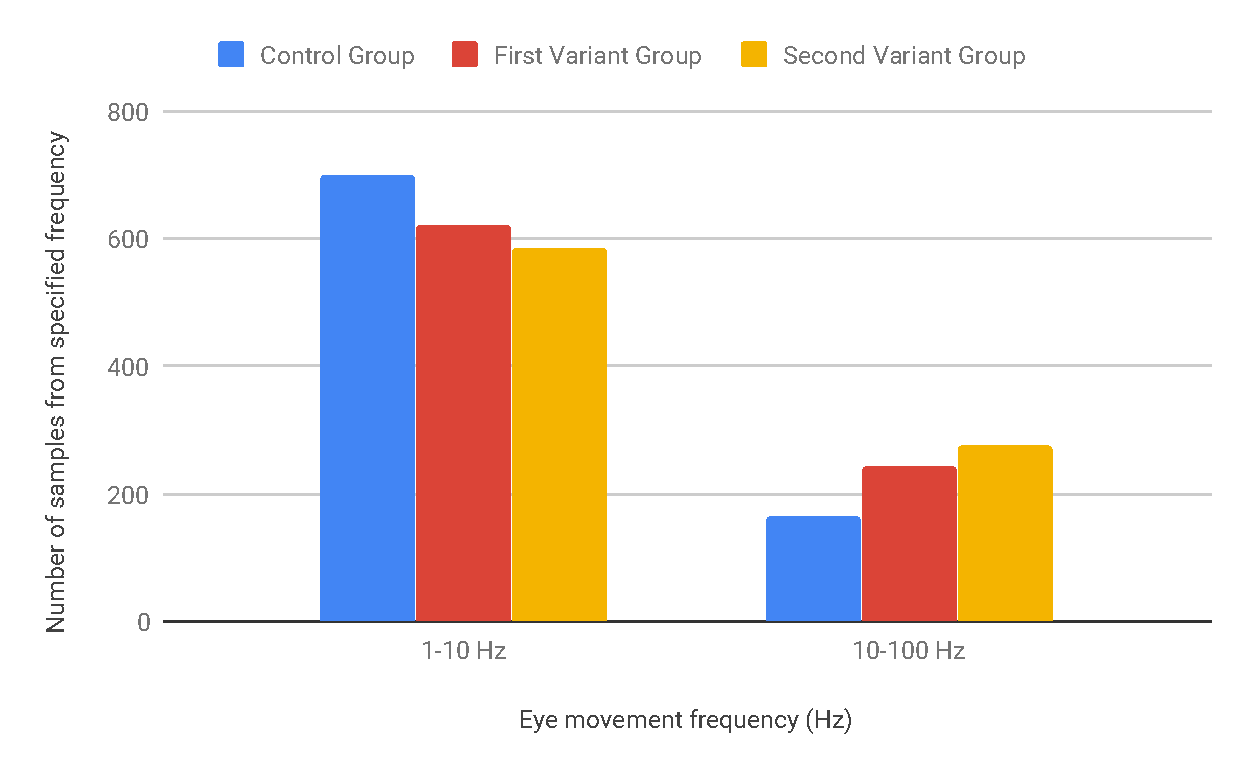
\includegraphics[width=\textwidth]{eye.pdf}
    \caption{Aggregate eye movement frequency per group. Slow eye movements are tracked in the 1-10 Hz range and faster eye movements are tracked within the 10-100 Hz range.}
    \label{fig:res_eye_movement}
\end{figure}

\paragraph{} \textbf{Brain-wave data}: We analyzed the brain-wave patterns of smartphone users over a period of 60 days, in which the analysis of the obtained data presented the percentages of each type of brain-wave, which in turn was used to infer the relative mental status of each group on an average. The brain-wave data indicated that the users when restricted access to their smartphones (shown by the first and second variant groups) show better REM (Rapid Eye Movement) sleep activity, which is an important factor in maintaining mental health\cite{basics2016understanding}. Moreover, there is a gradual increase in the percentage of gamma waves and beta waves, which imply that users are able to stay more focused on their current task without being susceptible to distractions. Another thing to note is that the proportions of alpha and delta waves even out\cite{hauri1973alpha}, which means that the sleep patterns are also made proper even if REM sleep is not to be factored in. From this we can infer that the dreamless sleep and heavy sleep states of the users mind are equalized when the restrictions are imposed.

\begin{table}[hbtp]
  \begin{center}
    \begin{tabular}{|r|c|c|c|}
    \hline
    \multirow{2}{*}{\textbf{\begin{tabular}[c]{@{}r@{}}Percentage of\\ brain waves\end{tabular}}} & \multicolumn{3}{c|}{\textbf{Group}}                                 \\ \cline{2-4} 
                                                                                                  & \textbf{Control} & \textbf{First variant} & \textbf{Second variant} \\ \hline
    Alpha waves                                                                                   & 20               & 24                     & 18                      \\ \hline
    Beta waves                                                                                    & 20               & 26                     & 30                      \\ \hline
    Gamma waves                                                                                   & 5                & 6                      & 8                       \\ \hline
    Delta waves                                                                                   & 35               & 30                     & 19                      \\ \hline
    Theta waves                                                                                   & 20               & 22                     & 25                      \\ \hline
    \end{tabular}
    \caption{Average percentages of brain waves of users of each group}
    \label{tab:tabtwo}
  \end{center}
\end{table}

\paragraph{} We need to observe the other studies that were conducted on the topic of excessive and/or compulsive usage of smartphones when attempting to derive meaning from the given results as well. There are multiple studies that prove that there is indeed a perceptible effect due to excessive and/or compulsive usage of smartphones \cite{haug2015smartphone, samaha2016relationships, mok2014latent}. However, the experiment conducted displays the effects of such usage of smartphones on mental health, which are seen from the variations in the levels of lethargy and attentiveness, which can be inferred from the above data. Certain studies also utilize applications to gauge the levels of smartphone usage and try to determine the negative effects of overuse of smartphones\cite{lin2015time, lin2017incorporation}, which is similar to what is attempted in this experiment, but the focus on brain-wave activity and the eye-movement patterns in this experiment display another facet of smartphone addiction; specifically the effects on the mental health and the resulting effects of the same.


\subsection{Experiment 2 : Testing efficiency of solution}

\paragraph{} To analyze the effectiveness of SageSense, we propose an experiment that measures how useful the solution is in reducing excessive and/or compulsive usage of smartphones. This is achieved by measuring the variance in the overall mental health levels of smartphone users that use SageSense, which is indicated by the brain-wave patterns collected from these users. To conduct this experiment, we collect brain-wave data of each user at two points in time; at the beginning of the experiment before the user starts to use SageSense, and at the completion of the experiment, which is the mark at which the user completes 60 days of its continued usage. The data collection done at both these points in time is run for a 24-hour frame, to gain the complete brain-wave activity of the users over a whole day. Conducting analysis over the data collected thus will provide an insight into the user's day-to-day usage patterns and mental health status, which can then be used to draw a comparison between mental health levels before and after using SageSense. This will then provide the basis to conclude whether the solution we propose is effective or not.

\subsubsection{Research Data}

\paragraph{} This experiment attempts to contrast the user's states of mental health and overall usage of his/her smartphone before and after using SageSense for a fixed time period (60 days). To accomplish the same, we collect two main kinds of data from each participant of the experiment, which are:

\begin{itemize}
    \item Brain-wave activity, which includes the following:
    \begin{itemize}[label=$\ast$]
        \item Delta waves (.5 - 3 Hz)
        \item Theta waves (3 - 8 Hz)
        \item Alpha waves (8 - 12 Hz)
        \item Beta waves (12 - 38 Hz)
        \item Gamma waves (38 - 42 Hz)
    \end{itemize}
    \item Smartphone usage patterns, which includes time spent on smartphone
\end{itemize}

\paragraph{} We utilize the same guidelines formulated in the first experiment (based on \citeauthor{buzsaki2006rhythms}'s work\cite{buzsaki2006rhythms}) to analyse the trends in the brain-wave data recorded from each participant. The smartphone usage patterns are mainly used to perceive the relative improvement the participant has made in terms of curbing excessive and/or compulsive usage of his/her smartphone.

\subsubsection{Experimental Setup}

\paragraph{} Since the experiment aims to measure the effectiveness of SageSense, it becomes the main component of the experiment system. The application records smartphone usage patterns by running in the background as a service. The wearable subsystem of SageSense provides a method to record each participant's brain-wave activity. The wearable headband records brain-wave activity in real-time and sends it to the application which locally processes the data on the smartphone itself, which then provides dynamic lockout timeframes to the user. In the consumer version of SageSense, there is no dependence on any external servers. However, for the purposes of data aggregation, the participants use a modified version of SageSense that records the two kinds of data mentioned above, and sends the recorded data to respective database instances running on a data collection server.

\subsubsection{Research Design}

\paragraph{} The experiment was conducted on a multi-ethnic group of 500 participants (Ethnicity: 20\% North American, 45\% Asian, 25\% African and 10\% Australian; Gender: 51\% male, 49\% female; Age: 18-24 - 37\%, 25-40 - 41\%, 41-50 - 22\%). These participants were divided into two groups on the criteria that each group consisted of an equal number of participants whose usage when taken on an average should roughly equal (allowing tolerance of +/-0.5 hours) that of the other group. The first group became the control group, which consisted of 250 participants and the second group became the variant group, which consisted of 250 participants. Participants of the control group are not given the chance to use SageSense's ability to deliver lockout timeframes, and are allowed unrestricted access. However, participants of the variant group have this ability enabled, effectively restricting the usage of their smartphones over the duration of the experiment (60 days).

\paragraph{} The experiment requires that each instance of data collection done should be over a span of 24 hours, so that the complete set of patterns and variations of brain-wave activity and smartphone usage can be recorded. Additionally, a constraint was also placed on the participants that they should complete 60 days of continuous usage. Failing this requirement would render the data collected from the participant invalid.

\subsubsection{Data Collection}

\paragraph{} We collect two kinds of data from each participant; the brain-wave activity and the smartphone usage patterns. Both these types of data are collected from each participant at two points in time; at the start of the experiment and at the end of the experiment. Each instance of data collection is run for 24 hours. The data collection is done using a data collection server that hosts two database instances. The modified version of SageSense used in this experiment sends the recorded data to these database instances. One database instance records the brain-wave data, and the other records the usage patterns. The complete data is finally downloaded from the server, and we finally compare the data obtained from the control group and the variant group to measure the approximate measure of effectiveness of SageSense amongst the userbase.

\subsubsection{Results and Discussion}

\paragraph{} Since the experiment deals with two types of data collected from each participant i.e. the brain-wave activity and the smartphone usage patterns, the results are presented in accordance with the results that were obtained from each type of data. The brain-wave activity results display the user's mental status while the smartphone usage patterns display the time that each participant spends on his/her smartphone.

\begin{table}[hbtp]
  \begin{center}
    \begin{tabular}{|r|c|c|}
    \hline
    \multirow{2}{*}{\textbf{Smartphone usage (in hours)}} & \multicolumn{2}{c|}{\textbf{Group}} \\ \cline{2-3} 
                                                          & \textbf{Control} & \textbf{Variant} \\ \hline
    Before using SageSense                                & 5.71             & 5.87             \\ \hline
    After using SageSense                                 & 4.93             & 2.14             \\ \hline
    \end{tabular}
    \caption{The average usage duration of participants in each group (on a daily basis)}
    \label{tab:tabthree}  
  \end{center}
\end{table}

\paragraph{} \textbf{Smartphone usage patterns}: SageSense was provided to both the participating groups, but only the variant group had the functionality of lockout timeframes enabled. This wasn't available in the version installed on the participants of the control group. From Figure \ref{fig:udcon} and \ref{fig:udvar}, it is surprising to find that all the participants have shortened usage spans, which imply that all the participants have cut down on their smartphone usage. This was expected in the variant group, since SageSense delivered lockout timeframes to the participants in the variant group, but the users in the control group have quantifiable (albeit noticeably lesser) improvement as well. We infer that this is due to the fact that the participants are now aware of their time spent on their smartphone and have made a conscious attempt to reduce their smartphone usage due to SageSense reporting them on the time that they spent on their phones. This inference also explains the consistent reduction in the short usage spans across both the groups.

\begin{figure}[hbtp]
    \centering
    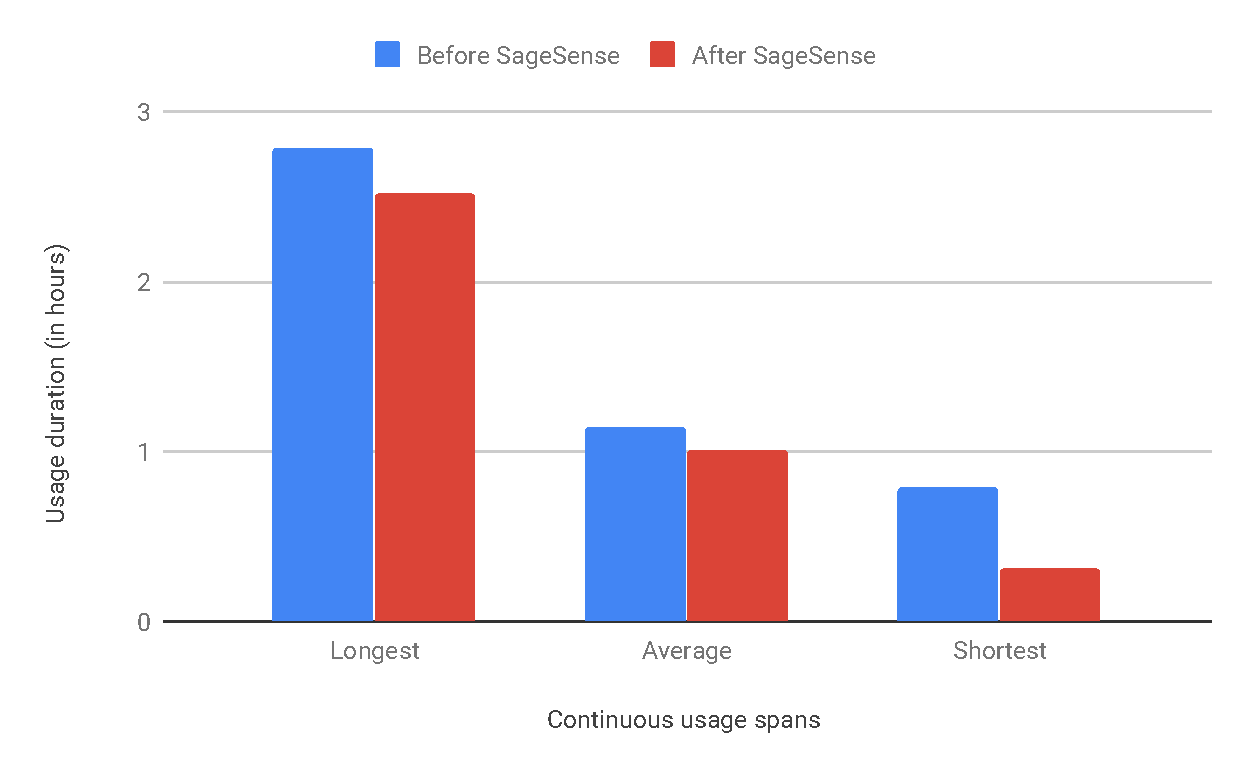
\includegraphics[width=\textwidth]{ud-control.pdf}
    \caption{The longest, average and shortest continuous smartphone usage spans of the control group}
    \label{fig:udcon}
\end{figure}

\begin{figure}[hbtp]
    \centering
    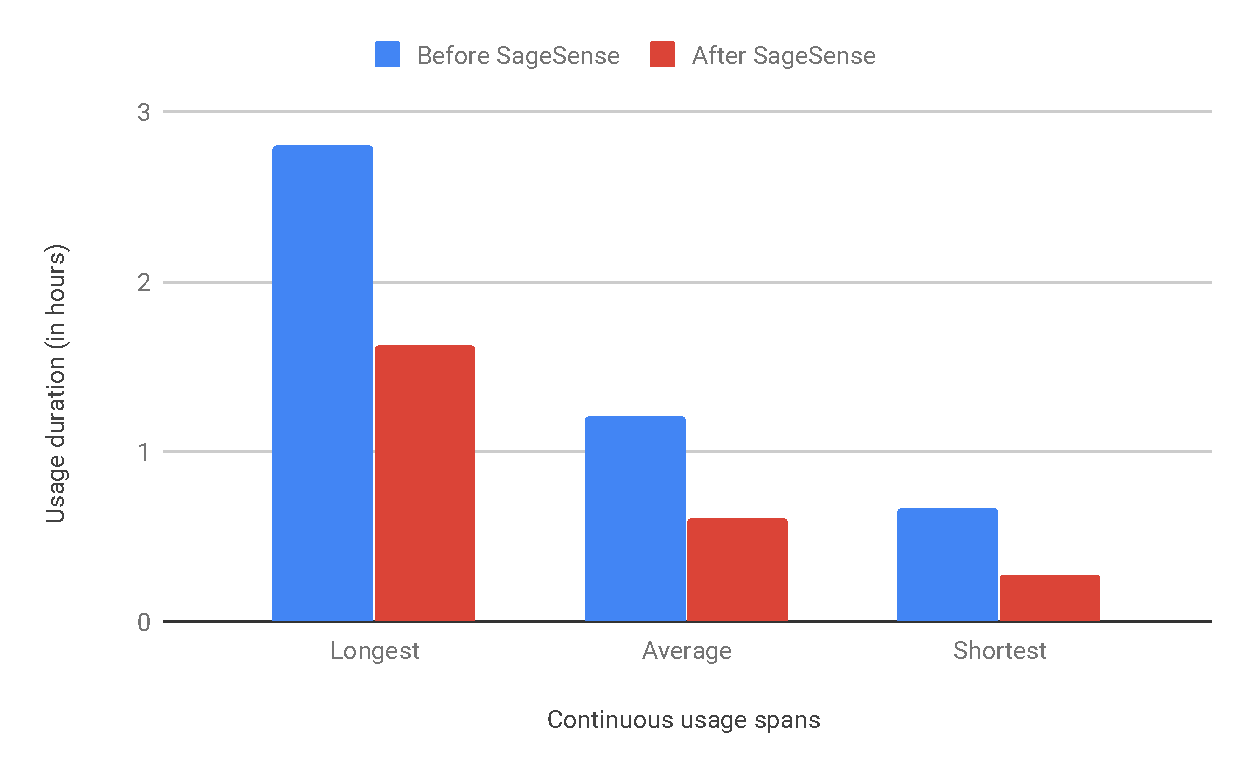
\includegraphics[width=\textwidth]{ud-variant.pdf}
    \caption{The longest, average and shortest continuous smartphone usage spans of the variant group}
    \label{fig:udvar}
\end{figure}

\paragraph{} \textbf{Brain-wave activity}: The results of the brain-wave activity analysis is displayed in Table \ref{tab:tabfour}. On drawing a comparison between the changes in aggregate brain-wave patterns between the start and end of the participants of the control group, we see that there is no visible difference in the same. However, drawing the same comparison on the variant group gives us a perceptible change wherein we can see three things:

\begin{itemize}
    \item The percentage of the alpha and delta waves try to equalize themselves.
    \item There is a decrease in the percentage of beta waves when comparing the two points.
    \item There is an increase in the percentage of gamma and theta waves when comparing the two points.
\end{itemize}

\paragraph{} The equalization of alpha and delta waves can be attributed to the return of the participants' sleep levels to the optimum, since both light and heavy (dreamless) sleep states proportions are made equal now. The increase in the percentage of gamma and theta waves indicate the increase in the user's levels of concentration and increase in attention span. The decrease in beta waves denote the decrease in the time the user is in the near-sleep/dozing off state, wherein the user lacks attention and constantly drifts off.

\begin{table}[hbtp]
\centering
\begin{tabular}{|r|c|c|c|c|}
\hline
\multirow{2}{*}{\begin{tabular}[c]{@{}r@{}}Percentage of\\ brain-wave activity\end{tabular}} & \multicolumn{2}{c|}{Control group} & \multicolumn{2}{c|}{Variant group} \\ \cline{2-5} 
                                                                                             & Start            & End             & Start            & End             \\ \hline
Alpha waves                                                                                  & 19.60            & 19.80           & 19.51            & 17.86           \\ \hline
Beta waves                                                                                   & 19.90            & 19.96           & 20.14            & 28.65           \\ \hline
Gamma waves                                                                                  & 5.47             & 5.39            & 5.32             & 8.61            \\ \hline
Delta waves                                                                                  & 34.93            & 33.72           & 35.01            & 18.98           \\ \hline
Theta waves                                                                                  & 20.10            & 21.13           & 20.02            & 25.60           \\ \hline
\end{tabular}
\caption{Brain-wave activty (in percentage) over 24-hour periods at the beginning and end of the experiment}
\label{tab:tabfour}
\end{table}

\section{Conclusion}

\paragraph{} Smartphones are undoubtedly one of the better products of innovation in the computing field, which was not only developed as a communication device, but also as a irreplaceable tool to consume media and get work done, among other capabilities. They have now grown to be the hub to the ever-growing connected world. However, the research that we conduct shows that these tiny devices are also heralds, if not the agents of a variety of mental health issues. These health issues include lack of sleep, depression, lack of concentration and lethargy. While there are a myriad of existing solutions that try and tackle this problem, we believe that they are ineffective at delivering personalized lockout timeframes without manual user intervention, which then puts the control in the user's hands. Thus, we devised our application SageSense that builds a system of providing lockout timeframes based on real-time analysis of brain-wave activity and eye movement data. We also measured the effectiveness of SageSense and thus, we were able to validate our claim of it being superior to existing application-based solutions that provide lockout timeframes. With our testing of the application's effectiveness, we see that restriction of smartphone usage among its users tends to provide its users with a better state of mind than without the application. Going forward, we see a future of smartphone users who are either addicted to their smartphone, or rely heavily on a similar control mechanism like SageSense to restrict themselves from overusage. Either way, we feel that this is not a complete solution, since users will then be overdependent on their smartphones either way. Thus, we call for our fellow researchers to understand the urgency of the situation, and unite as a scientific community to bring awareness to the general population about the detrimental effects of smartphones, by which every user can find his/her level of optimistic use and thereby be free from depending on a brain of silicon.

\clearpage
\bibliographystyle{plainnat}
\bibliography{cite}

\end{document}